
%(BEGIN_QUESTION)
% Copyright 2010, Tony R. Kuphaldt, released under the Creative Commons Attribution License (v 1.0)
% This means you may do almost anything with this work of mine, so long as you give me proper credit

This ``lift station'' pump control circuit has a problem.  The sump pump is supposed to come on when the high level is reached, and turn off when the water pumps down to the low level point.  Instead, however, the motor ``cycles'' on and off at the high-level point.

$$\includegraphics[width=15.5cm]{i03844x01.eps}$$

Using an AC voltmeter, you measure a voltage from point {\bf D} to point {\bf E} that switches back and forth between 120 volts and 0 volts.

\vskip 10pt

Identify the likelihood of each specified fault for this circuit.  Consider each fault one at a time (i.e. no coincidental faults), determining whether or not each fault could independently account for {\it all} measurements and symptoms in this circuit.

% No blank lines allowed between lines of an \halign structure!
% I use comments (%) instead, so that TeX doesn't choke.

$$\vbox{\offinterlineskip
\halign{\strut
\vrule \quad\hfil # \ \hfil & 
\vrule \quad\hfil # \ \hfil & 
\vrule \quad\hfil # \ \hfil \vrule \cr
\noalign{\hrule}
%
% First row
{\bf Fault} & {\bf Possible} & {\bf Impossible} \cr
%
\noalign{\hrule}
%
% Another row
High level switch failed open &  &  \cr
%
\noalign{\hrule}
%
% Another row
Low level switch failed open &  &  \cr
%
\noalign{\hrule}
%
% Another row
Broken wire between {\bf D} and M1 coil &  &  \cr
%
\noalign{\hrule}
%
% Another row
Contactor auxiliary contact failed open &  &  \cr
%
\noalign{\hrule}
%
% Another row
480 volt fuse(s) blown &  &  \cr
%
\noalign{\hrule}
%
% Another row
Contactor main contact(s) failed open &  &  \cr
%
\noalign{\hrule}
%
% Another row
Broken wire between {\bf B} and {\bf G} &  &  \cr
%
\noalign{\hrule}
%
% Another row
Thermal overload unit tripped &  &  \cr
%
\noalign{\hrule}
%
% Another row
Low level switch failed shorted &  &  \cr
%
\noalign{\hrule}
%
% Another row
Transformer secondary winding failed open &  &  \cr
%
\noalign{\hrule}
} % End of \halign 
}$$ % End of \vbox

Finally, identify the {\it next} diagnostic test or measurement you would make on this system.  Explain how the result(s) of this next test or measurement help further identify the location and/or nature of the fault.

\underbar{file i03844}
%(END_QUESTION)





%(BEGIN_ANSWER)

% No blank lines allowed between lines of an \halign structure!
% I use comments (%) instead, so that TeX doesn't choke.

$$\vbox{\offinterlineskip
\halign{\strut
\vrule \quad\hfil # \ \hfil & 
\vrule \quad\hfil # \ \hfil & 
\vrule \quad\hfil # \ \hfil \vrule \cr
\noalign{\hrule}
%
% First row
{\bf Fault} & {\bf Possible} & {\bf Impossible} \cr
%
\noalign{\hrule}
%
% Another row
High level switch failed open &  & $\surd$ \cr
%
\noalign{\hrule}
%
% Another row
Low level switch failed open &  & $\surd$ \cr
%
\noalign{\hrule}
%
% Another row
Broken wire between {\bf D} and M1 coil &  & $\surd$ \cr
%
\noalign{\hrule}
%
% Another row
Contactor auxiliary contact failed open & $\surd$ &  \cr
%
\noalign{\hrule}
%
% Another row
480 volt fuse(s) blown &  & $\surd$ \cr
%
\noalign{\hrule}
%
% Another row
Contactor main contact(s) failed open &  & $\surd$ \cr
%
\noalign{\hrule}
%
% Another row
Broken wire between {\bf B} and {\bf G} & $\surd$ &  \cr
%
\noalign{\hrule}
%
% Another row
Thermal overload unit tripped &  & $\surd$ \cr
%
\noalign{\hrule}
%
% Another row
Low level switch failed shorted &  & $\surd$ \cr
%
\noalign{\hrule}
%
% Another row
Transformer secondary winding failed open &  & $\surd$ \cr
%
\noalign{\hrule}
} % End of \halign 
}$$ % End of \vbox


%(END_ANSWER)





%(BEGIN_NOTES)

If the motor cycles on and off at the high-level point, it means the seal-in contact is not doing its job to latch the motor control circuit on.

\vskip 20pt \vbox{\hrule \hbox{\strut \vrule{} {\bf Virtual Troubleshooting} \vrule} \hrule}

This question is a good candidate for a ``Virtual Troubleshooting'' exercise.  Presenting the diagram to students, you first imagine in your own mind a particular fault in the system.  Then, you present one or more symptoms of that fault (something noticeable by an operator or other user of the system).  Students then propose various diagnostic tests to perform on this system to identify the nature and location of the fault, as though they were technicians trying to troubleshoot the problem.  Your job is to tell them what the result(s) would be for each of the proposed diagnostic tests, documenting those results where all the students can see.

During and after the exercise, it is good to ask students follow-up questions such as:

\begin{itemize}
\item{} What does the result of the last diagnostic test tell you about the fault?
\item{} Suppose the results of the last diagnostic test were different.  What then would that result tell you about the fault?
\item{} Is the last diagnostic test the best one we could do?
\item{} What would be the ideal order of tests, to diagnose the problem in as few steps as possible?
\end{itemize}

%INDEX% Troubleshooting review: electric circuits

%(END_NOTES)

